% fig_mc_aggregate.tex  — bare tikzpicture for \input in main_report8.tex
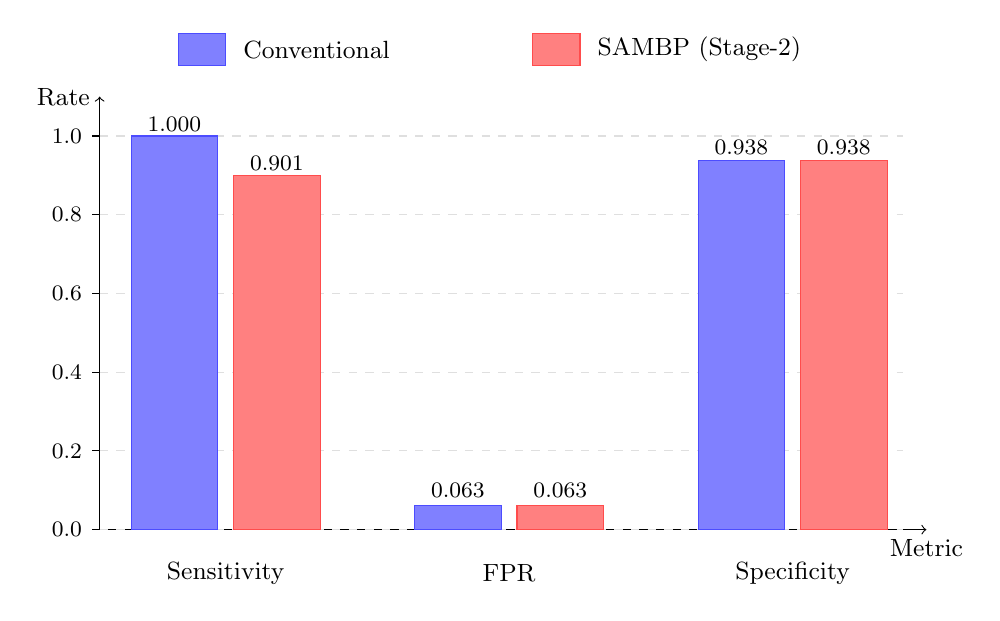
\begin{tikzpicture}

\def\H{5.0}   % height = 100%

% Axes
\draw[->] (0,0) -- (0,\H+0.5) node[left,font=\small]{Rate};
\draw[->] (0,0) -- (10.5,0)   node[below,font=\small]{Metric};

% Y-axis ticks and horizontal grid
\foreach \y/\val in {0/0.0, 1.0/0.2, 2.0/0.4, 3.0/0.6, 4.0/0.8, 5.0/1.0}{
    \draw (0,\y) -- (-0.1,\y) node[left,font=\footnotesize]{\val};
    \draw[gray!25,dashed] (0,\y) -- (10.2,\y);
}

% ---- Group 1: Sensitivity ----
% Conv = 1.000 -> height 5.0
\fill[blue!50]  (0.4,0) rectangle (1.5,5.0);
\draw[blue!70]  (0.4,0) rectangle (1.5,5.0);
% SAMBP = 0.9006 -> height 4.503
\fill[red!50]   (1.7,0) rectangle (2.8,4.503);
\draw[red!70]   (1.7,0) rectangle (2.8,4.503);
\node[font=\footnotesize] at (0.95,5.15)  {1.000};
\node[font=\footnotesize] at (2.25,4.65)  {0.901};
\node[font=\small,align=center] at (1.6,-0.55) {Sensitivity};

% ---- Group 2: FPR ----
% Conv = 0.0625 -> height 0.3125
\fill[blue!50]  (4.0,0) rectangle (5.1,0.3125);
\draw[blue!70]  (4.0,0) rectangle (5.1,0.3125);
% SAMBP = 0.0625 -> height 0.3125
\fill[red!50]   (5.3,0) rectangle (6.4,0.3125);
\draw[red!70]   (5.3,0) rectangle (6.4,0.3125);
\node[font=\footnotesize] at (4.55,0.5)  {0.063};
\node[font=\footnotesize] at (5.85,0.5)  {0.063};
\node[font=\small,align=center] at (5.2,-0.55) {FPR};

% ---- Group 3: Specificity ----
% Conv = 0.9375 -> height 4.6875
\fill[blue!50]  (7.6,0) rectangle (8.7,4.6875);
\draw[blue!70]  (7.6,0) rectangle (8.7,4.6875);
% SAMBP = 0.9375 -> height 4.6875
\fill[red!50]   (8.9,0) rectangle (10.0,4.6875);
\draw[red!70]   (8.9,0) rectangle (10.0,4.6875);
\node[font=\footnotesize] at (8.15,4.85) {0.938};
\node[font=\footnotesize] at (9.45,4.85) {0.938};
\node[font=\small,align=center] at (8.8,-0.55) {Specificity};

% ---- Legend ----
\fill[blue!50] (1.0,\H+0.9) rectangle (1.6,\H+1.3);
\draw[blue!70] (1.0,\H+0.9) rectangle (1.6,\H+1.3);
\node[right,font=\small] at (1.7,\H+1.1) {Conventional};

\fill[red!50] (5.5,\H+0.9) rectangle (6.1,\H+1.3);
\draw[red!70] (5.5,\H+0.9) rectangle (6.1,\H+1.3);
\node[right,font=\small] at (6.2,\H+1.1) {SAMBP (Stage-2)};

\end{tikzpicture}
